\chapter{10neV parxkaraNa}

\centerline{{\rm\bfseries MULTIPLICATION.}}
\vskip .3cm

\centerline{{\large\bf guNAkAravu.}}
\smallskip


guNAkAraveMdare oMdeV vidhavAda leKaKxgaLanunx kelavu sAri sheVrisidare Aguva oTaTxnanx tiLiyapaDisatakakxdudx. idu saMkalanada saMkeSxVpa riVtiyAgirutatxde.

hAyxgeMdare--- $4+4+4+4+4+4$ nAlukx I aMkiyanunx ArAvatiR baradu kUDisidare $24$ Agutatxde. Adare adu guNAkAradalilx $4\times6=24$ hiVgAgutatxde.

hAgeyeV $7$nunx eMTAvatiR baradu kUDisidare ELeMTulx $56$ eMdAgutatxde.

\noindent guNayx  $\Box$ idu guNisi koLaLx takakx saMKeya hesaru.\\ 
guNaka $\Box$ idu guNisuva saMKayxda hesaru.\\
labadhx athavA guNAkAra $\Box$ idu guNisida meVle baruva Palada hesaru\\

\begin{center}
{\large\bf karxmavu.}
\end{center}
\begin{longtable}{|>{$}c<{$}|>{$}c<{$}|>{$}c<{$}|}
\hline
1 \times 1 = 1 & 2 \times 1 = 2 & 3 \times 1 = 3\\
1 \times 2 = 2 & 2 \times 2 = 4 & 3 \times 2 = 6\\
1 \times 3 = 3 & 2 \times 3 = 6 & 3 \times 3 = 9\\
1 \times 4 = 4 & 2 \times 4 = 8 & 3 \times 4 = 12\\
1 \times 5 = 5 & 2 \times 5 = 10 & 3 \times 5 = 15\\
1 \times 6 = 6 & 2 \times 6 = 12 & 3 \times 6 = 18\\
1 \times 7 = 7 & 2 \times 7 = 14 & 3 \times 7 = 21\\
1 \times 8 = 8 & 2 \times 8 = 16 & 3 \times 8 = 24\\
1 \times 9 = 9 & 2 \times 9 = 18 & 3 \times 9 = 27\\
1 \times 10 = 10 & 2 \times 10 = 20 & 3 \times 10 = 30\\
\hline
4 \times 1 = 4 & 5 \times 1 = 5 & 6 \times 1 = 6\\
4 \times 2 = 8 & 5 \times 2 = 10 & 6 \times 2 = 12\\  
4 \times 3 = 12 & 5 \times 3 = 15 & 6 \times 3 = 18 \\ 
4 \times 4 = 16 & 5 \times 4 = 20 & 6 \times 4 = 24\\  
4 \times 5 = 20 & 5 \times 5 = 25 & 6 \times 5 = 30\\  
4 \times 6 = 24 & 5 \times 6 = 30  & 6 \times 6 = 36 \\ 
4 \times 7 = 28 & 5 \times 7 = 35 &  6 \times 7 = 42\\
4 \times 8 = 32 & 5 \times 8 = 40 &  6 \times 8 = 48\\
4 \times 9 = 36 & 5 \times 9 = 45 &   6 \times 9 =52\\ 
4 \times 10 = 40 & 5 \times 10 = 50 &  6 \times 10 =60\\
\hline
7 \times 1 =7 &  8 \times 1 = 8 & 9 \times 1 = 9\\
7 \times 2 =14 &  8 \times 2 = 16 & 9 \times 2 = 18\\
7 \times 3 =21 &  8 \times 3 = 24 & 9 \times 3 = 27\\
7 \times 4 =28 &  8 \times 4 = 32 & 9 \times 4 = 36\\
7 \times 5 =35 &  8 \times 5 = 40 & 9 \times 5 = 45\\
7 \times 6 =42 &  8 \times 6 = 48 & 9 \times 6 = 54\\
7 \times 7 =49 &  8 \times 7 = 56 & 9 \times 7 = 63\\
7 \times 8 =56 &  8 \times 8 = 64 & 9 \times 8 = 72\\
7 \times 9 =63 &  8 \times 9 = 72 & 9 \times 9 = 81\\
7 \times 10 =70 & 8 \times 10 = 80 & 9 \times 10 = 90\\
\hline
10 \times 1 = 10 & 11 \times 1 = 11 & 12 \times 1 = 12\\ 
10 \times 2 = 20 & 11 \times 2 = 22 & 12 \times 2 = 24\\ 
10 \times 3 = 30 & 11 \times 3 = 33 & 12 \times 3 = 36\\ 
10 \times 4 = 40 & 11 \times 4 = 44 & 12 \times 4 = 48\\ 
10 \times 5 = 50 & 11 \times 5 = 55 & 12 \times 5 = 60\\ 
10 \times 6 = 60 & 11 \times 6 = 66 & 12 \times 6 = 72\\ 
10 \times 7 = 70 & 11 \times 7 = 77 & 12 \times 7 = 84\\ 
10 \times 8 = 80 & 11 \times 8 = 88 & 12 \times 8 = 96\\ 
10 \times 9 = 90 & 11 \times 9 = 99 & 12 \times 9 = 108\\ 
10 \times 10 = 100 & 11 \times 10 = 110 & 12 \times 10 = 120\\
\hline 
\end{longtable}


\begin{center}
{\large\bf sUtarx.}
\end{center}

\begin{verse}
kaM|| guNayxda aMkigaLelalxva| guNakada Ekadali guNisi barigere keLagaM|| guNakada dashakAdigaLiM|\break guNisutatxda (sonenxnaLidadxre)radarasathxLadi bariyuta kUDeY||\\

kaM|| sonenxyoLaMkiyaniriya| losxnenxyadAguvadutiLidu dashigiVsahitaM|| naninxyiM bariyu\break muMdina| sonenxgaLelalxvanu labadhxdoLu taMdiriseY||\\

vi|| guNakada EkasAthxnada aMkiyiMda guNayxda aMkigaLanenxlAlx guNisi gereV keLage baradu koMDu, A meVle guNakada dasha shatAdayxMkigaLiMda guNisutatx labadhxgaLanunx AyAya sathxLada aMkigaLa sAthxnagaLa modalogxMDu keLage baradu kUDisabeVku. sonenxyiMda aMkiyanAnxgaliV, aMkiyiMda sonenxgaLanAnxgaliV guNisidare sonenxyeV baruvadeMdu tiLidu adakekx muMce guNisida aMkiya dashagiV sameVtavAgi bariyabeVku. muMdina aMdare---guNayxda madhayxdalilx hecAcxgiruva sonenxgaLanUnx matUtx guMNayx guNakagaLa muMde iruva sonenxgaLanUnx labadhxdalilx tegadu baradukoLaLxbeVku.
\end{verse}

\newpage

\begin{center}
{\large\bf hAyxgeMdare.}

\medskip
\begin{tabular}{>{$}c<{$}l}
1050 & guMNayx\\ 
 260 & guNaka\\
\cline{1-1}
 \quad630\\
210 \\
\cline{1-1}
273000 & guNAkAra\\
\cline{1-1}
\end{tabular}
\end{center}

idaralilx guMNayx guNakagaLa EkasAthxnagaLalilx sonenxgaLiruvadadxriMda adara guNAkAra sonenxyAguvadu. AdadxriMda adariMda guNisadeV biTuTx biTuTx dashakasAthxnadalilxruva $6$riMda guNisalu $6\times5=30$ Ayitu. meVlina guNAyxMkiya $5$ra Ace sonenx yiruvadadxriMda A sathxLadalilx dashagi sahitavAda $30$neV baradirutatxde. A meVle $6\times1=6$ idanunx baradirutatxde. taruvAya $2\times5=10$ hatatxkekx hatUtx eMdu $10$nunx adara sAthxnavAda eraDaneV aMkiya keLage baradirutatxde matutx $2\times1=2$ eraDoMdulx $2$ eraDanunx baradirutatxde. matutx avugaLanunx kUDisalAgi $2730$ Ayitu, idara muMde guMNayx guNakagaLa muMdugaDeyiruva eraDu sonenxgaLanunx bariyalu $273000$ labadhxvAyitu, ideV guNAkAravu.
\begin{center}
\begin{tabular}{>{$}c<{$}l}
2050 & guMNayx\\ 
 107& guNaka\\
\cline{1-1}
\quad 1435\\
205\\
\cline{1-1}
219350 & guNAkAra\\
\cline{1-1}
\end{tabular}
\end{center}

idaralilx guNakada Eka sAthxnadiMda pArxraMBisalu ELeYdalu $35$ Ayitu $35$kekx $35,$ eMdu dashigiV sahita baradirutatxde. A meVle, ELeraDalu $14$nunx baradide. muMde dashasAtxnadalilx sonenx iruvadadxriMda adariMda guNisadeV biTuTx biTiTxrutatxde. taruvAya shatasAthxnadalilxruva $1$riMda guNisi adara sathxLavAda mUraneV aMkiV keLaginiMdA baradu kUDisalAgi $21935$ Ayitu, idara muMde guNayxdalilx muMdeyiruva oMdu sonenxyanunx baradukoLaLxlu $219350$ labadhxvAyitu.

\begin{center}
{\large\bf tALe}
\end{center}

\begin{verse}
kaM|| aLiguMNayxva navadiMdali| vuLuvaninxriNaka navadoLaLeduLuviMdaM|| aLiyada navadiMduLidudu| tiLi labadhxvanavadoLaLedaruLuvinasamanaM||\\

vi|| guMNayxvanunx navadiMda aLadu uLuvanunx (guNakavanunx navadiMdaLadare uLiyuva saMKayxdiMda) guNisi A labadhxvanunx navadiMdaLadare uLiyuva sheVSavu (labadhxvanunx navadiMdA aLadare uLiyuva sheVSakekx) sariyAgidadxre guNAkAradalilx tapipxlalxveMbudakekx sAkiSx uMTu. hAyxgeMdare, Iga guNayxvu $3476\times$ guNakavu $5342=$ labadhxvu $18568792$ Adare, tALeyanunx noVDa takakx karxmavu. guNayxvanunx $9$riMdA aLiyalu sheVSavu $2\times$ guNakavanunx $9$riMdA aLada sheVSavu $5=10$ idanunx $9$riMdA aLadare sheVSavu $1$ idu labadhxvanunx $9$riMda aLadare uLiyuva $1$ kekx sariyAgiruvadadxriMda leKaKxdalilx tapipxlalxveMbudakekx sAkiSx uMTu. athavA guNAkAra labadhxvanUnx guMNayxdiMda BAgisidare, guNaka labadhxkUkx A guNakadiMda bAgisidare guMNayxlabadhxkekx sariyAgirabeVku.\\
\end{verse}

\begin{center}
{\large\bf KaMDa guNAkAravu.}
\end{center}

KaMDa guNakAraveMdare guNakAMkiyanunx eraDu, athavA mUru KaMDagaLanAnxgi viMgaDisi parxteyxVka KaMDagaLiMda guNisuva sulaBavAda riVtiyu. idaralilx kUDisa takakxdudx ilalxdadxriMda sulaBavAgiruvadu.

\begin{center}
{\large\bf sUtarx.}
\end{center}

\begin{verse}
kaM|| guNakave KaMDirxsu manabaM| danitanuguNisalekx guNaka sariyAguva pari| guNisuta KaMDoMdaroLuM| enitAguva labadhxvanunx matotxMdaroLuM||\\

vi|| guNakAMkiyanunx manasusx baMda hAge eraDu athavA mUru KaMDagaLanunx mADa beVku. hAyxgeMdare A KaMDagaLanenxlAlx parasapxravAgi guNisidare guNakAMkiya labadhxkekx sariyAgirabeVku. AmeVle, modalaneV KaMDadiMda guNisi A labadhxvanunx matotxMdu KaMDadiMdalU A labadhxvanunx inonxMdu KaMDadiMdalU guNisi bariya beVku.\\
\end{verse}

\begin{center}
{\large\bf hAyxgeMdare.\\
\vskip .2cm
\boldmath{$1245$} idanunx \boldmath{$24$}riMda guNisu.}
\end{center}
\begin{equation*}
\left.
\begin{aligned}
\text{hAyxgeMdare, guNayx $(2+0+5+0)=7$}\\
\text{guNaka $(1+0+7)=8$}
\end{aligned}
\right\}
\end{equation*}
$=7\times8=56$ idanunx navadiMda aLadare $2$ uLiVtu. idu guNAkAravAda $(2+1+3+5)=11-9=2$ I sheVSa sariyAgide. AdadxriMdA tapipxlalxvu.

ililx guNaka $24$ra KaMDagaLAyxvAyxveMdare,---
\begin{equation*}
\left.
\begin{aligned}
(1)\; & 6\times4=24\\
(2)\; & 8\times3=24\\
(3)\; & 2\times3\times4=24\\
(4)\; & 2\times2\times6=24\\
(5)\; & 12\times2=24
\end{aligned}
\right\}
\quad\text{I riVti KaMDagaLuMTAgutatxve.}
\end{equation*}

avugaLalilx yAvadAdarU oMdu tarada KaMDAMkigaLiMda guNisidAgUyx labadhxgaLu oMdeV vidhavAgi $24$ riMda pUNaR guNAkAravanunx mADidadxkekx sariyAgi baruvavu.

\eject

\begin{center}
{\large\bf riVtiyu.}
\end{center}

\begin{center}
\begin{tabular}{rrrr}
\begin{tabular}[t]{>{$}c<{$}>{$}c<{$}}
\multicolumn{1}{c}{$(1)$}\\[5pt]
1245 & \text{guMNayx}\\
\quad\quad 6 & \text{modalaneV KaMDavu}\\
\cline{1-1}
7470 & \text{labadhxvu}\\
\quad\quad 4 & \text{eraDaneV KaMDavu}\\
\cline{1-1}
29880 & \text{guNAkAravu}\\
\cline{1-1}
\end{tabular} &
\begin{tabular}[t]{>{$}c<{$}l}
\multicolumn{1}{c}{$(2)$}\\[5pt]
1245\\
\quad\quad 8\\
\cline{1-1}
9960& \\
\quad\quad 3 &\\
\cline{1-1}
29880 & labadhxvu\\
\cline{1-1}
\end{tabular} &
\begin{tabular}[t]{>{$}c<{$}l}
\multicolumn{1}{c}{$(3)$}\\[5pt]
1245\\
\quad\quad 2\\
\cline{1-1}
2490&\\
\quad\quad 3 &\\
\cline{1-1}
7470 & \\
\quad\quad 4 & \\
\cline{1-1}
29880 & labadhxvu\\
\cline{1-1}
\end{tabular} 
\end{tabular}\\[20pt]


\begin{tabular}{>{$}l<{$}}
(4)\; 1245\times2=2490\times2=4980\times6=29880\\
(5)\; 1245\times12=14940\times2=29880
\end{tabular} 
\end{center}

\medskip

\begin{center}
{\large\bf 6neV aBayx udAharaNegaLu.}
\end{center}

\begin{tabular}{>{$}l<{$}>{$}l<{$}>{$}l<{$}}
(1)\; 1234\times12 & (7)\; 2342\times42 & (13)\; 6452\times63\\
(2)\; 14050\times24 & (8)\; 3545\times45 & (14)\; 4634\times72\\
(3)\; 1548\times16 & (9)\; 9435\times49 & (15)\; 5543\times81\\
(4)\; 1654\times28 & (10)\; 4683\times56 & (16)\; 7425\times96\\
(5)\; 3546\times32 & (11)\; 4536\times54 & (17)\; 15432\times48\\
(6)\; 2456\times36 & (12)\; 3542\times64 & (18)\; 954026\times144\\
\end{tabular}

\medskip

\begin{center}
{\large\bf 7neV aBayx udAharaNe pUNaR guNAkAragaLu.}
\end{center}


\begin{tabular}{>{$}l<{$}>{$}l<{$}>{$}l<{$}}
(1)\; 1543\times427 & (7)\; 7080\times6050 & (13)\; 708095\times6070\\
(2)\; 5430\times563 & (8)\; 54000\times23500 & (14)\; 2548002\times76740\\
(3)\; 1542\times2436 & (9)\; 18040\times2080 & (15)\; 152207\times146\\
(4)\; 5425\times6384 & (10)\; 25402\times7416 & (16)\; 304414\times803\\
(5)\; 2547\times3068 & (11)\; 1963000\times1200 & (17)\; 456621\times219\\
(6)\; 5040\times3020 & (12)\; 90030\times8005 & (18)\; 608828\times292\\
\end{tabular}\\[2pt]

\begin{tabular}{>{$}l<{$}}
(19)\; 154+562-125\times72-8+6\\
(20)\; 265+423\times148+524-2\\
(21)\; 694\times762+185-201+56\times9\\
(22)\; 719+432\times315-612+4\times8\\
(23)\; 918-246+128\times216+64-32\\
(24)\; 1025\times3476+112-6\times2
\end{tabular}

\medskip

\begin{center}
{\bf\Large {pUvaRda AcaraNeyalilxdadx manegaLa guNAkAravu.}}
\vskip .3cm

{\large\bf sUtarx.}
\end{center}

\begin{verse}
kaM|| irutihaguNayxda guNakada| parimitigaMmaneya baradu mUlege reVKisu| pariviDideVkAdigaLiM| diridiridadabaradu kUDu mUlegaLarituM||\\
vi|| guMNayx guNakAMkigaLa parimitige sariyAgi manegaLanunx nimiRsi, A manegaLa meVlina BAgadalilx guMNAyxMkigaLanUnx eDagaDeV BAgadalilx guNakAMkigaLanUnx oMdoMdu manege oMdoMdaMkigaLiruvaMteV baradu, A manegaLalilx mUlege sariyAgi reVKegaLanunx baradu, guNakada modalaneV aMkiyiMdalU A meVle eraDaneV mUraneV itAyxdi aMkigaLiMdalU guNisi guNisi A manegaLalilx dashagaLa sameVtavAgi baradu, mUleV sAlugaLanunx kUDisabeVku.
\end{verse}

\begin{center}
{\large\bf hAyxgeMdare.}
\end{center}


\begin{center}
$345\times426$
\end{center}
\vskip -.7cm
\begin{figure}[h]
\centering
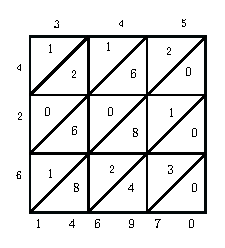
\includegraphics[scale=1.2]{mu.eps}
\end{figure}

idaralilx guMNayxdalilx mUraMkigaLU guNakadalilx mUraMkigaLU iruva kAraNa avugaLige sariyAda mane\-gaLanunx nimiRsi, mUlege geregaLa baradu, vidhi parxkArakekx meVlABxgadalilx guMNAyxMkigaLanUnx eDagaDeyalilx guNakAMkiya labadhxvanUnx baradirutatxde.

modalu guMNayxda EkasAthxnada aMki $6$riMda guMNayxda EkasAthxnadaMki $5$nunx guNisi $30$nUnx keLagina kaDeV mane\-yalilxyU anaMtara guMNayxda dashasAthxnada $4$nunx guNisi $24$nunx adariVceV maneyalilx baradirutatxde. taruvAya guMNayxda shatasAthxnada aMki $3$nunx guNisi $12$nunx adariVceV maneyalilx baradirutatxde. idaraMteyeV guNakada dasha, shatasAthxnadaMkigaLiMda guNisi, AyA sAlina manegaLalilx baradu kUDisalu $146970$ iSuTx guNAkAravAgirutatxde.

\begin{center}
{\large\bf 8neV aBayx udAharaNe.}
\end{center}

\begin{tabular}{>{$}l<{$}|>{$}l<{$}}
(1)\; 3335\times5321 & (4)\; 4315\times207\\
(2)\; 24254\times1248 & (5)\; 3458\times1050\\
(3)\; 545\times637\\
\end{tabular}

\medskip

\begin{center}
{\large\bf 9neV aBayx udAharaNe.}
\end{center}

\begin{enumerate}[\rm(1)]
\item $1$ maNa yAlakikxge $4525$ rUpAyi karxyavAdare $528$ maNagaLigeSuTx karxya?

\item obabx manuSayxnu parxti divasavU $25$ meYlugaLaMte $500$ divasagaLalilx eSuTx meYlugaLa parxyANavanunx mADAyxnu?

\item $1$ duDiDxge $25$ mAvina haMNugaLAdare $1$ rUpAyige eSuTx haMNugaLu baMdAvu?

\item obabxnu $1$ duDiDxge $12$ haMNugaLa parxkArakekx $10$ duDiDxgU, $15$ haMNugaLa parxkArakekx $11$ duDiDxgU, $18$ haMNugaLa parxkArakekx $24$ duDiDxgU tegadukoMDu adaralilx tananx heMDatige $30$ haMNUgaLanUnx maganige $25$ haMNugaLanUnx magaLige $20$ haMNugaLanUnx koTuTx, $50$ haMNugaLanunx mAridanu. Adare avanalilx inUnx eSuTx haMNugaLira beVku?

\item oMdu Urinalilx $50$ viSuNx deVvAlayavu $75$ shivAlayagaLU idadxvu. oMdoMdu deVvAsAthxnadalilx parxti\break divasavU $180$ diVpagaLa parxkArakekx $3$ tiMgaLU $15$ divasagaLu hatitxsutAtx baMdare, oTuTx eSuTx diVpagaLAguvavu?

\item obabx huDuganalilx $10$ duDUDx inonxbabxnalilx $1$ pAvaliyU itutx. avaribabxrU $1$ kAsige $5$ bALe haMNugaLa parxkArakekx tegadukoMDaru. Aga A vAyxpAragAranalilx inUnx $200$ haMNugaLu uLadidadxvu. Adare avanu modalu taMdidadx haMNugaLeSuTx?

\item obabx huDuganalilx $1$ pAvaliyU inonxbabxnalilx $2$ adhaR rUpAyigaLu idadxvu. modalaneVyavanu duDiDxge $8$ra hAgU, eraDaneVyavanu duDiDxge $12$ra hAgU mAvina haMNugaLanunx tegadukoMDaru. Aga modalaneVyavanigiMyalU eraDaneVyavanige eSuTx haMNugaLu hecAcxgi baMdavu heVLu? \hfill u. $480$ haMNugaLu

\item obabxnu aMgaDiyalilx dara sheVrige $5$ duDiDxna hAge $1$ maNa yaMNeyanunx $1$ dhaDiya tupapxvanunx $3$ paMceVru saKaKxreyanunx tegadukoMDanu. Aga avanu aMgaDiyavanige eSuTx duDuDxgaLanunx koDabeVku heVLu? 

\hfill u. $325$ duDuDxgaLu. 

\item oMdu divasakekx $60$ GaLigegaLu athavA $24$ GaMTegaLu athavA $12$ laganxgaLU Agidadxre $1$ tiMgaLige yAvAyxvadeSeTxSATxguvadu? 

\hfill u.$1800$ GaLige, $720$ GaMTe, $360$ laganxgaLu.

\item obabx meVsitxrXyu kuciR dara $1$ kekx $3$ rUpAyina hAge $48$ kuciRgaLanUnx meVju $1$kekx $5$ rUpAyina hAge $31$ meVjugaLanUnx peTiTxgekekx $4\frac{1}{2}$ rUpAyina hAge $12$ peTiTxgegaLanUnx maMca $1$kekx $15$ rUpAyiya hAge $11$ maMcagaLanUnx mAribiTaTxnu. Aga avanige eSuTx rUpAyigaLu barabeVku? \hfill u. $518$ rUpAyi.                   

\end{enumerate}
